The agent will be an autonomous program acting as a special user that looks at the raw data stream and existing metadata from the remote repository and generates new metadata which is pushed back into the repository. The metadata is any processed data that the system needs to serve its purpose, such as congestion data, heat maps and new routes.

\subsubsection{Agent Requirements}\mbox{}\\
\begin{figure} 
  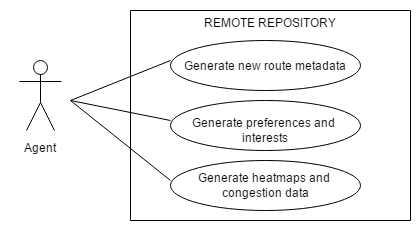
\includegraphics[width=\textwidth]{diagrams/Specific_Requirements/Agent_Use_Case.png}
\end{figure}

\\
\bigskip

\FuncReq
{Generate new heat maps and congestion data}
{Trivial}
{The agent is authenticated and has sufficient privileges to perform its job.}
{Trivial}

\FuncReq
{Generate new route metadata}
{The agent can process raw location data from the remote repository to learn new routes through campus. Because of this, the workload of data capture is reduced since older students and lectureres on campus will map the routes out for the system by simply walking their usual routes through campus.}
{The agent is authenticated and has sufficient privileges to perform its job.}
{Trivial}

\FuncReq
{Generate preferences and interests}
{There will be an agent that learns the preferences and interests of the data-subjects from existing metadata and the raw data stream from the remote repository.}
{The agent is authenticated and has sufficient privileges to perform its job.}
{Trivial}
 
